
\begin{TP}[Eponge de Menger]

\partie{Réalisation}

\begin{enumerate}
 \item Réalisez 20 cubes identiques en papier d'arêtes 4 cm.
 \item Placez ces 20 copies de telle façon qu'elles forment un nouveau cube de 12 cm d'arêtes  sans les parties centrales. Comme le dessin ci-dessous :
 \begin{center} 
\includegraphics[width=2.8cm]{menger1} \end{center}
 \begin{center} Étape 1 \end{center}
 \item Regroupez toutes les copies des cubes réalisées et complétez leurs nombres pour en avoir 400. Placez ces 400 copies de telle façon qu'elles forment un nouveau cube de 36 cm d'arêtes  sans les parties centrales. Comme le dessin ci-dessous :
 \begin{center} 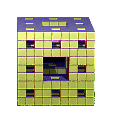
\includegraphics[width=2.8cm]{menger2} \end{center}
 \begin{center} Étape 2 \end{center}
 \item Combien de cubes seraient nécessaire pour construire la 3\up{ème} étape ? Quelle hauteur atteindrait l'éponge de Menger ?
 \begin{center} 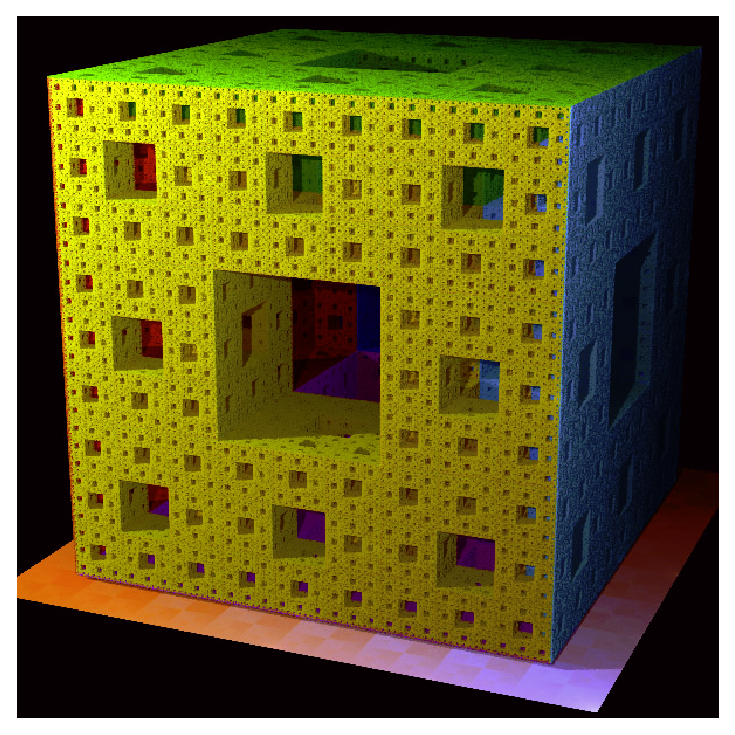
\includegraphics[width=8cm]{menger3} \end{center}
 \qquad \qquad \qquad \qquad \qquad \qquad \qquad \qquad \qquad \qquad \small{\emph{(Wikipedia, auteur : Solkoll)}}
 \end{enumerate}

\partie{Volumes}

La construction d'une éponge de Menger peut être décrite de la manière suivante :
\begin{itemize}
 \item Débuter par un cube ;
 \item Réduire le cube au tiers et en faire 20 copies ;
 \item Placer ces copies de telle façon qu'elles forment un nouveau cube de la même taille que l'original, sans les parties centrales ;
 \item Répéter le processus à partir de l'étape 2 pour chacun des 20 cubes ainsi créés.
 \end{itemize} 
Le solide obtenu à la limite, après un nombre infini d'itérations, est l'éponge de Menger.
\begin{enumerate}
 \item Que vaut le volume de l'étape 0, si on prend un cube d'arête 9 cm ?
 \item Que vaut le volume de l'étape 1 ? l'étape 2 ? et l'étape 3 ?
 \item Que dire du volume à l'étape 10 ? et 100 ?
 \item Que peut-on conclure ?
 \end{enumerate}
Ci-dessous, une éponge de Menger, coupée par un plan transversal passant par les milieux des six côtés du cube.
 \begin{center} 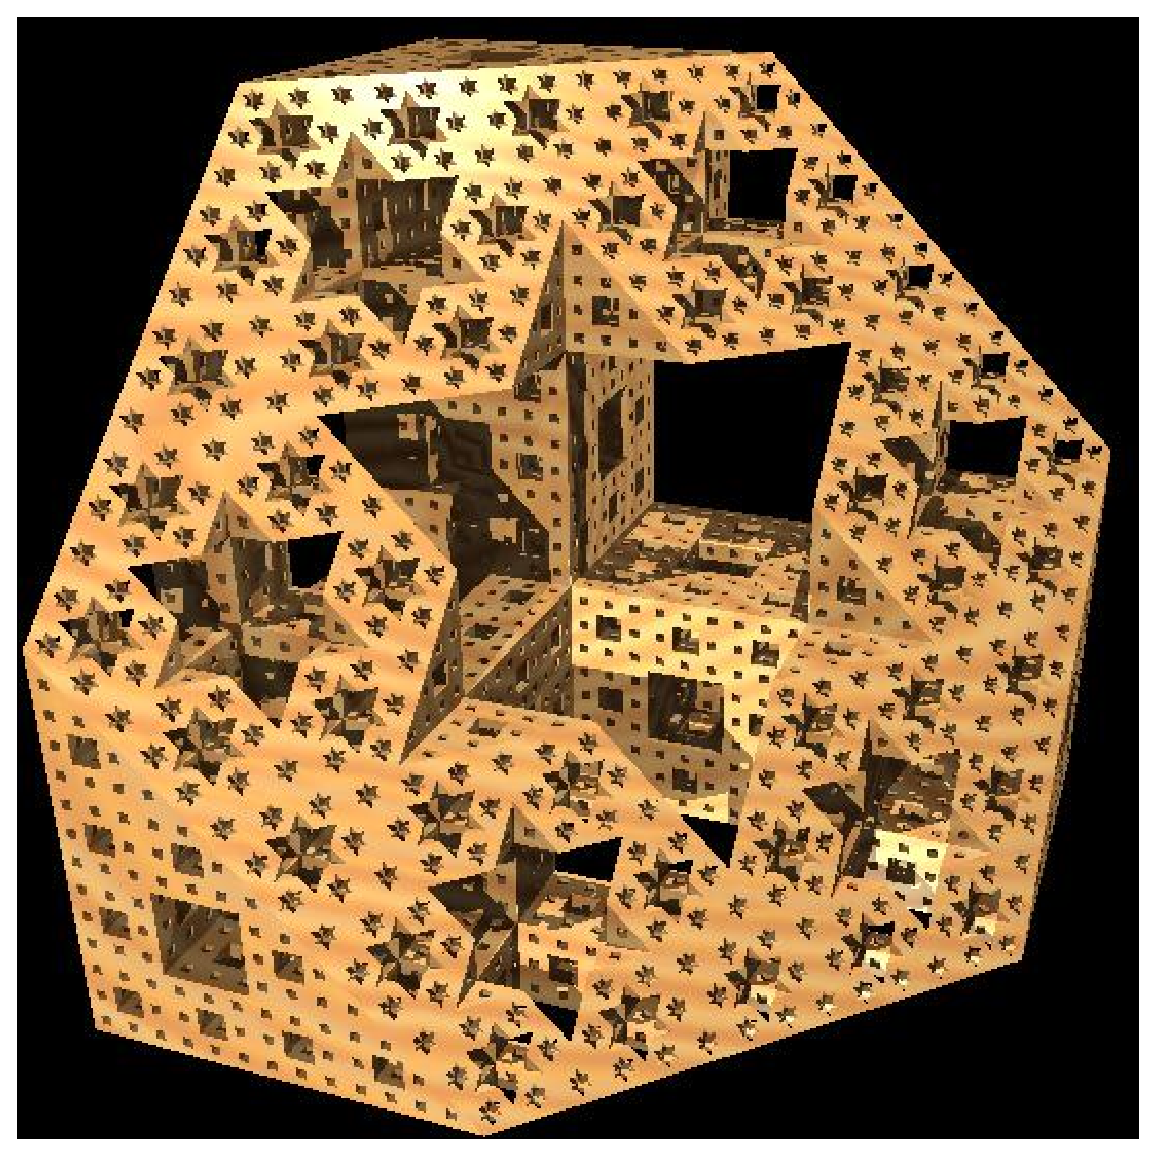
\includegraphics[width=8cm]{menger4} \end{center}
 \qquad \qquad \qquad \qquad \qquad \qquad \qquad \qquad \qquad \qquad \small{\emph{((Wikipedia, auteur : Theon)}}
 
\end{TP}

